\documentclass[tikz,border=2]{standalone}
\usetikzlibrary{decorations.pathreplacing,shadows,arrows,shapes,positioning,calc,backgrounds,fit,automata}

\definecolor{RED}{HTML}{E41A1C}
\definecolor{BLUE}{HTML}{377EB8}
\definecolor{GREEN}{HTML}{4DAF4A}
\begin{document}
\newcommand{\layersep}{1cm}
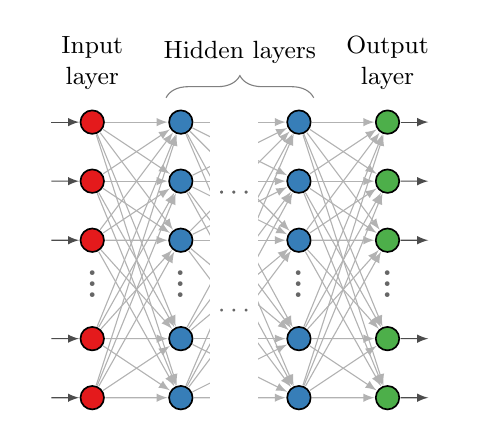
\begin{tikzpicture}[scale=0.75,draw=black!50, node distance=\layersep]
\tikzstyle{every pin edge}=[<-,shorten <=1pt]
\tikzstyle{myEdge}=[draw=black!30,>=latex, shorten >=.2pt, shorten <=.2pt]
\tikzstyle{vertex}=[draw=black,inner sep=3pt,semithick],
\tikzstyle{input neuron}=[vertex,circle,fill=RED];
\tikzstyle{output neuron}=[vertex,circle, fill=GREEN];
\tikzstyle{hidden1 neuron}=[vertex,circle, fill=BLUE];
\tikzstyle{hidden2 neuron}=[vertex,circle, fill=BLUE];
\tikzstyle{annot} = [text width=4em, text centered, font=\small]

\newcommand{\nodecolumn}[3]{
\foreach \y in {1,2,3}
\node[#1] (#2\y) at (#3,-\y) {};
\node[black!60] at (#3,-3.6) {\huge $\vdots$};
\foreach \y in {4,5}
\node[#1,shift={(0,-.5)}] (#2\y) at (#3,-\y) {};
}

\newcommand{\coledges}[2]{
\foreach \x in {1,...,5}
    \foreach \y in {1,...,5}
    \draw[myEdge,->] (#1\x) -- (#2\y);
}

\nodecolumn{input neuron}{inNeuron}{0}
\nodecolumn{hidden1 neuron}{hidden1}{1.5}
\nodecolumn{hidden2 neuron}{hidden2}{3.5}
\nodecolumn{output neuron}{outNeuron}{5}

\coledges{inNeuron}{hidden1}
\coledges{hidden1}{hidden2}
\coledges{hidden2}{outNeuron}

\foreach \x in {1,...,5}
    \draw[myEdge,black!70,<-] (inNeuron\x) -- +(-.7,0); 

\foreach \x in {1,...,5}
    \draw[myEdge,black!70,->] (outNeuron\x) -- +(.7,0); 

\def\y{0}
\node[annot] at (0,\y) {Input layer};
%% \node[annot] at (2,\y) {Hidden layer 1};
%% \node[annot] at (4,\y) {Hidden layer 2};
\node[annot] at (5,\y) {Output layer};

\draw[fill=white,shift={(0,.5)},draw=none] (2,-1) rectangle (2.8,-6.2);
\node[black!60] at (2.4,-4.2) {$\cdots$};
\node[black!60] at (2.4,-2.2) {$\cdots$};
\node[black!60] at (2.4,-2.2) {$\cdots$};
\draw [gray,decorate,decoration={brace,amplitude=8pt,raise=-4pt},yshift=0pt]
(1.25,-.4) -- (3.75,-.4) node [midway,below,yshift=.7cm,black] {\small Hidden layers};
\end{tikzpicture}
\end{document}

\end{tikzpicture}
\end{document}
